%%This is a very basic article template.
%%There is just one section and two subsections.
\documentclass{article}

\usepackage{graphicx} 
\usepackage{float}
\usepackage{fancyhdr}
\usepackage{pdfpages}
\usepackage{pdflscape}
\usepackage{geometry}
\usepackage[utf8]{inputenc}



\begin{document}
\section*{3D Laser Scan}
\label{sonar}


\begin{table}[ht!]

	\begin{tabular}{r l l p{12cm} }
		
		\textcolor{gray}{Especificação} &&& 	{Forecast 3D Laser Spinning Assembly
		com LMS 511}\\
		\textcolor{gray}{Data} &&& 				{14/08/2015}\\
        \textcolor{gray}{Beneficiado} &&&		{ASI PRODUCTS} \\
        \textcolor{gray}{CNPJ} &&& 				{Internacional} \\
        \textcolor{gray}{Número Nota} &&& 		{Compra não realizada} \\
		\textcolor{gray}{Quantidade} &&& 		{1} \\
		\textcolor{gray}{Valor} &&& 			{U\$44.000,00} \\
		%TODO DATA SHEET
		\textcolor{gray}{Data Sheet} &&& 		{} \\
		%TODO CODIGO RASTREAMENTO
		\textcolor{gray}{Código de Rastreamento} &&& {---} \\

		\textcolor{gray}{Função no projeto} &&& {O Escâner Laser 3D será utilizado
		para identificar e localizar as pás da turbina em relação ao robô, para que
		seja possível um correto alinhamento para a realização do revestimento
		metalizado.} \\
		\textcolor{gray}{Razão da Escolha} &&& {Dentre os dispositivos analisados que
		possuem a especificação necessária para o projeto, o TODO da
		TODO apresentou TODO.
		 \begin{itemize}
		  \item \textbf {3D Forecast Laser System por U\$37.000,00}
		  \item MultiSense SL \$ 28.445,00 
		  \item Velodyne HDL-64E - Aguardando cotação.
		\end{itemize}}

	\end{tabular}
\end{table}

\subsection{Foto do Material}
\begin{figure}[H]
 \centering
 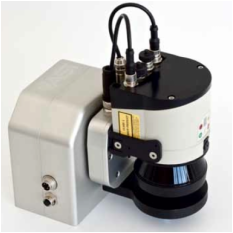
\includegraphics[width=0.4\columnwidth]{figs/forecast/foto.png}
 \caption{3D Forecast Laser System}
\end{figure}

\subsection{Foto do Material}
\begin{figure}[H]
 \centering
 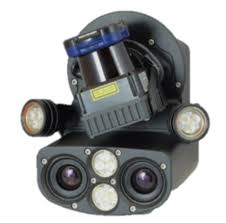
\includegraphics[width=0.4\columnwidth]{figs/multisense/multisense}
 \caption{3D Forecast Laser System}
\end{figure}



\subsection{Cotação 3D Forecast Laser System 1 }
\begin{figure}[H]
 \centering
 \includegraphics[page=3,width=1\columnwidth]{figs/forecast/quote1.pdf}
 \caption{Cotação Super Seaking DFP da Tritech}
\end{figure}

\subsection{Cotação MultiSense SL}
\begin{figure}[H]
 \centering
 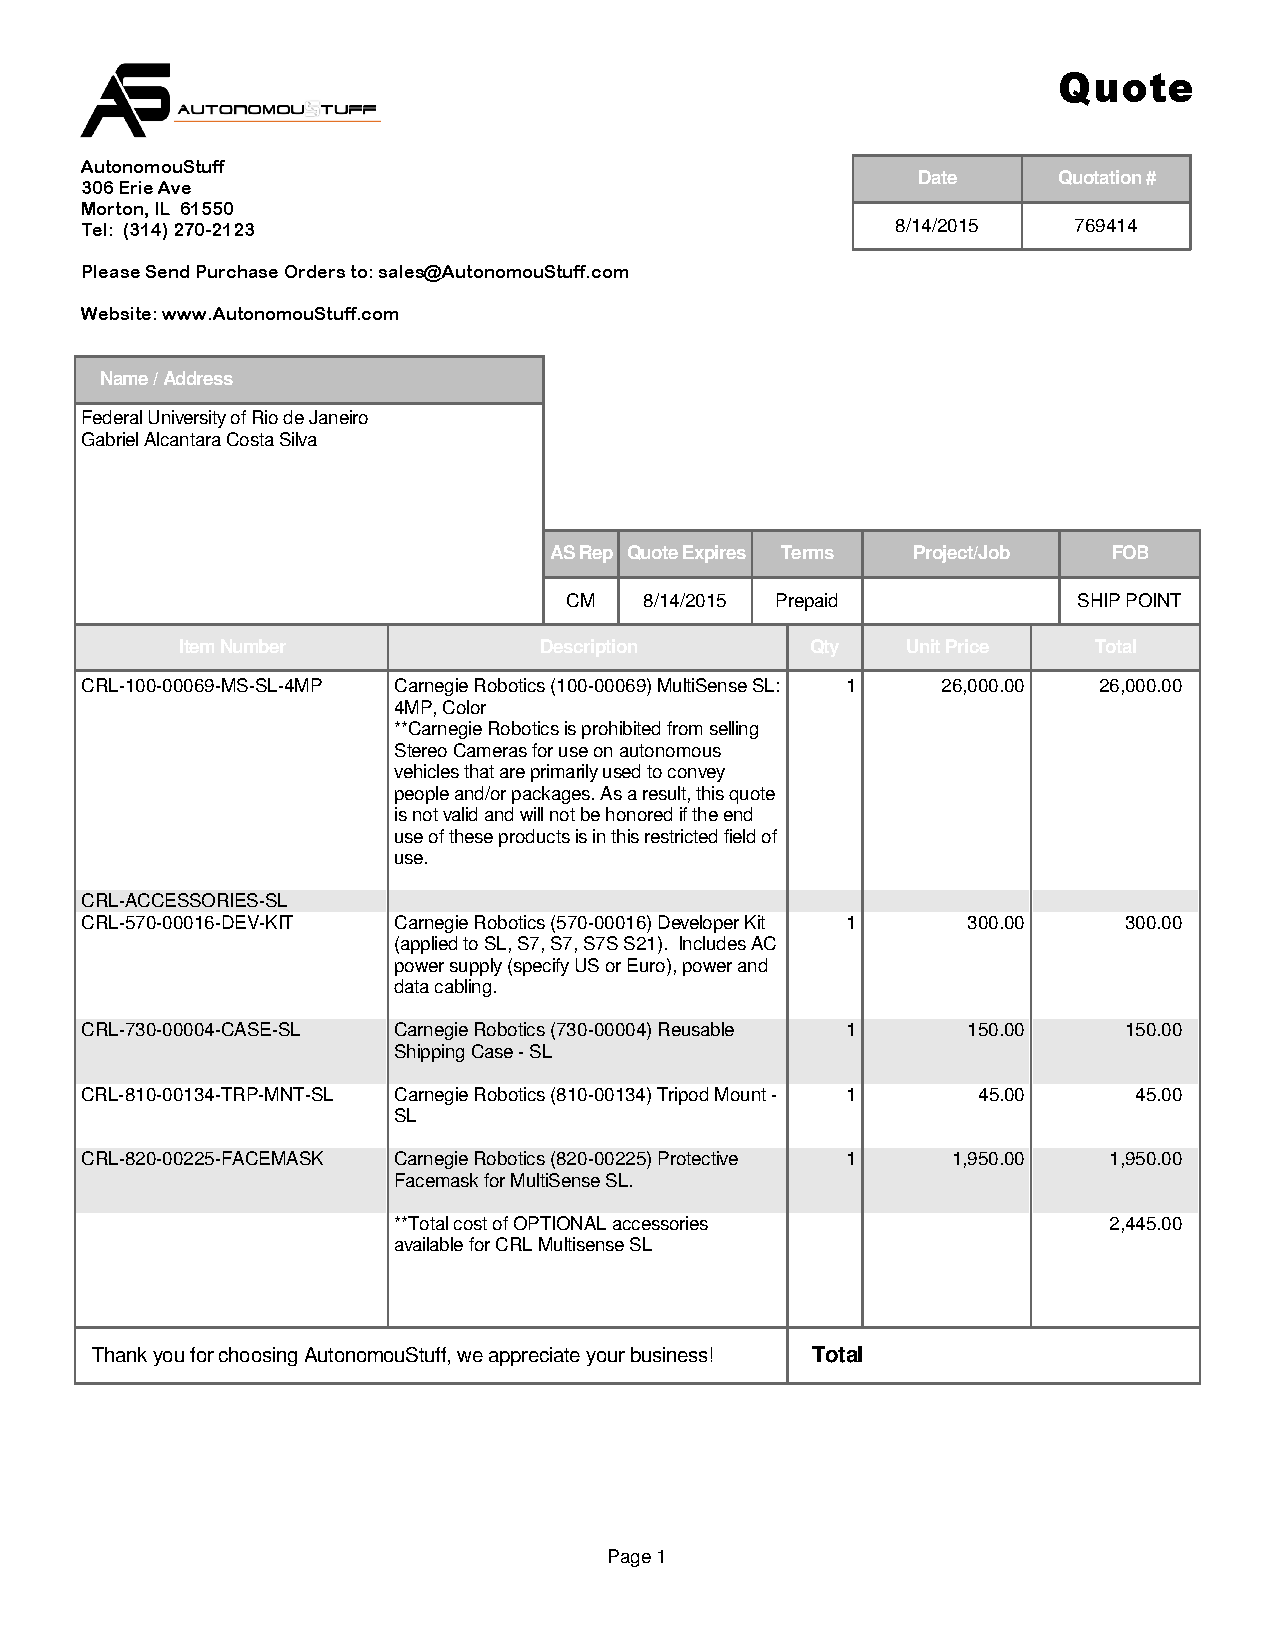
\includegraphics[page=1,width=1\columnwidth]{figs/forecast/quote2.pdf}
 \caption{Cotação Super Seaking DFP da Tritech}
\end{figure}

\begin{figure}[H]
 \centering
 \includegraphics[page=2,width=1\columnwidth]{figs/forecast/quote2.pdf}
 \caption{Cotação Super Seaking DFP da Tritech}
\end{figure}


\newpage

\section*{Point Laser}
\begin{table}[ht!]

	\begin{tabular}{r l l p{12cm} }
		
		\textcolor{gray}{Especificação} &&& 	{TODO}\\
		\textcolor{gray}{Data} &&& 				{14/08/2015}\\
        \textcolor{gray}{Beneficiado} &&&		{TODO} \\
        \textcolor{gray}{CNPJ} &&& 				{Internacional} \\
        \textcolor{gray}{Número Nota} &&& 		{Compra não realizada} \\
		\textcolor{gray}{Quantidade} &&& 		{1} \\
		\textcolor{gray}{Valor} &&& 			{TODO} \\
		%TODO DATA SHEET
		\textcolor{gray}{Data Sheet} &&& 		{} \\
		%TODO CODIGO RASTREAMENTO
		\textcolor{gray}{Código de Rastreamento} &&& {---} \\

		\textcolor{gray}{Função no projeto} &&& {O dispositivo de point laser tem o
		papel de servir de equipamento de segurança, assegurando uma distância mínima
		durante a operação do robô.}
		\\
		\textcolor{gray}{Razão da Escolha} &&& {TODO.
		 \begin{itemize}
		  \item TODO
		\end{itemize}}

	\end{tabular}
\end{table}

\end{document}
